\chapter[Deployment]{Deployment with Docker} \label{ch:deployment}

\section{Applicability of Containers}
Containers are becoming an ubiquituous technology. They help increase productivity, operational efficiency and deplyoment velocity while reducing infrastructure cost. As opposed to running several applications on a plain operating system or in a virtual machine, containers are far more flexible because they isolate their dependencies and libraries into their own environment. Containers sit on top of a physical server and its host OS while sharing the OS kernel. They are often compared to virtual machines which need hypervisors in order to virtualize and allocate hardware. Containers on the other hand share resources with the host OS which makes them very lightweight and cost efficient: they are usually only megabytes in size, whereas VMs need gigabytes to run. \autoref{fig:containervsvm} puts containers and VMs into a graphical contrast.

\begin{figure}[H]
    \begin{center}
    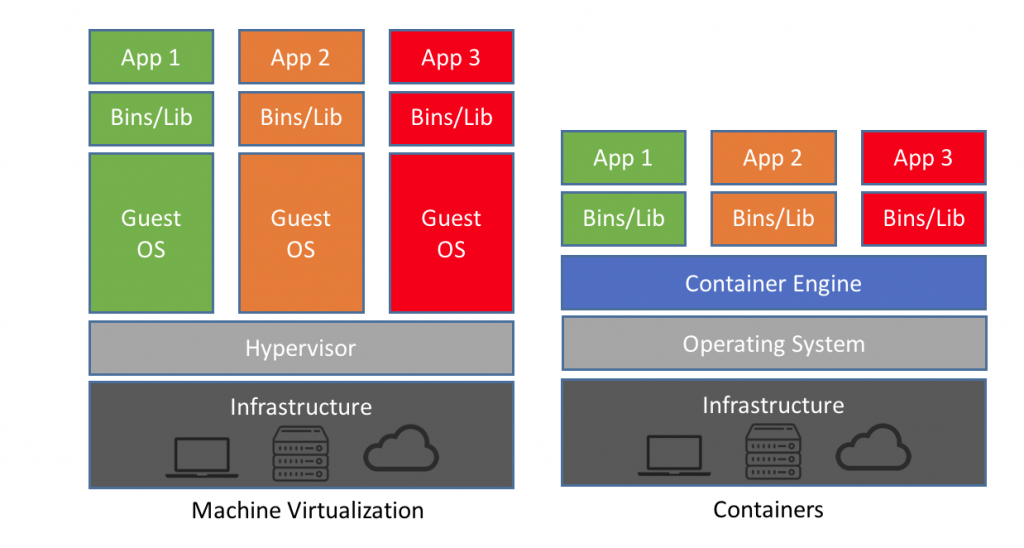
\includegraphics[width=\linewidth]{containervsvm}
    Source: \href{https://blog.netapp.com/wp-content/uploads/2016/03/Screen-Shot-2018-03-20-at-9.24.09-AM-1024x548.png}{blog.netapp.com}
    \end{center}
    \caption{Container vs VMs}
    \label{fig:containervsvm}
\end{figure}
  

\section{Docker}
Docker, the most widely used application level containerization technology advertises itself as a platform to "Build, Ship, and Run Any App, Anywhere".

\section{Docker Swarm}

\section{Microservices}

\section{Reverse Proxy}